\documentclass[green, compress]{beamer}
\usepackage[spanish, activeacute]{babel}
\usepackage[utf8]{inputenc}
\usepackage{beamerthemesplit}
\usepackage{beamerthemeshadow}
\usepackage{multirow}
\usepackage{tgpagella}
\usepackage{colores}

\usepackage{tikz} % Parar generar gráficos avanzados
\usetikzlibrary{arrows,decorations.markings}

\usetheme{Darmstadt}

\beamertemplateshadingbackground{orange!30}{white!80}

\useinnertheme{rounded}
\setbeamercovered{transparent}

\usecolortheme[named=verde]{structure}

\AtBeginSubsection[]
{
  \begin{frame}<beamer>
    \frametitle{Índice}
    \tableofcontents[currentsection,currentsubsection]
  \end{frame}

}

\title{\textit{GoM:} Simulador de batallas fantásticas}
\author[Aarón Bueno Villares]{Aarón Bueno Villares}

\begin{document}

\begin{frame}
	\titlepage
  % Fichero para incluir de forma rápida la licencia ne otros. Se
% distribuye junto a las imágenes de la licencia, en este caso
% cc-by-sa.
%
% Copyright (C) 2009 by Abrahán Fernández Nieto


\begin{center}
  
\includegraphics[scale=0.4]{imagenes/cc-by-sa.png}
\end{center}

%%% Local Variables: 
%%% mode: latex
%%% TeX-master: "../ejercicios"
%%% End: 

\end{frame}

\begin{frame}[allowframebreaks]{Índice}
  \tableofcontents
\end{frame}

\section{Introducción}
\begin{frame}{Batalla de Gaugamela}
\begin{center}
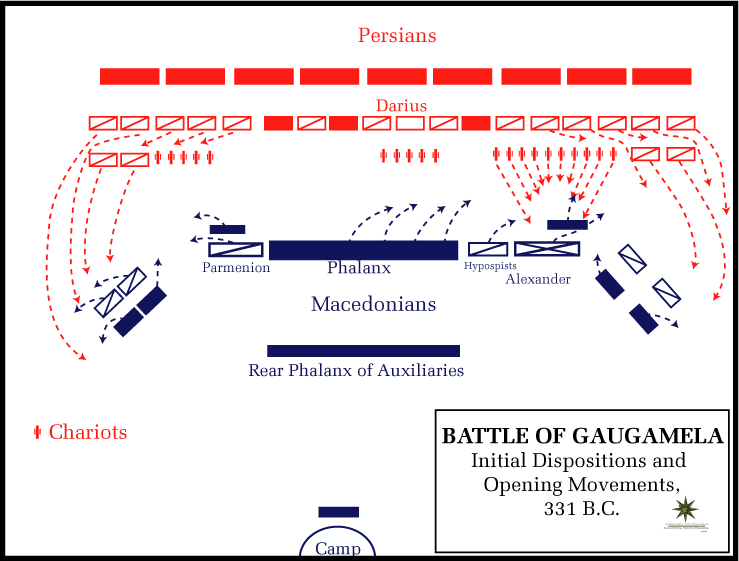
\includegraphics[scale=.3]{imagenes/gaugamela1.png}
\end{center}
\end{frame}

\begin{frame}{Batalla de Gaugamela}
\begin{center}
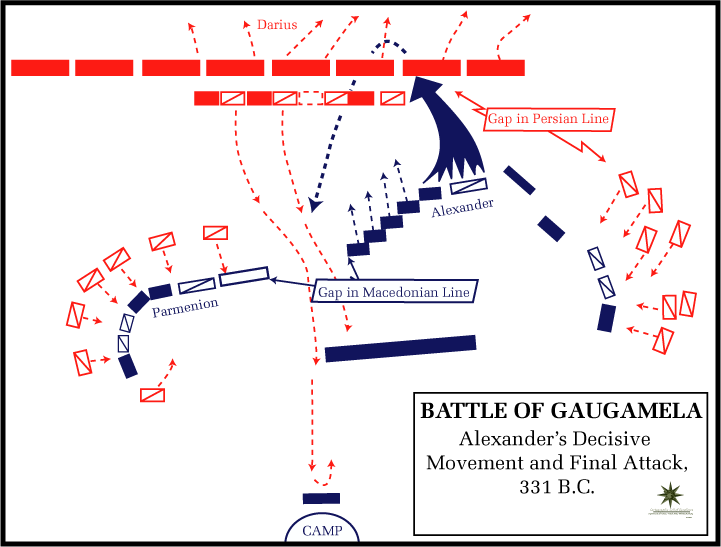
\includegraphics[scale=.3]{imagenes/gaugamela2.png}
\end{center}
\end{frame}

\begin{frame}{GoM}
\begin{center}
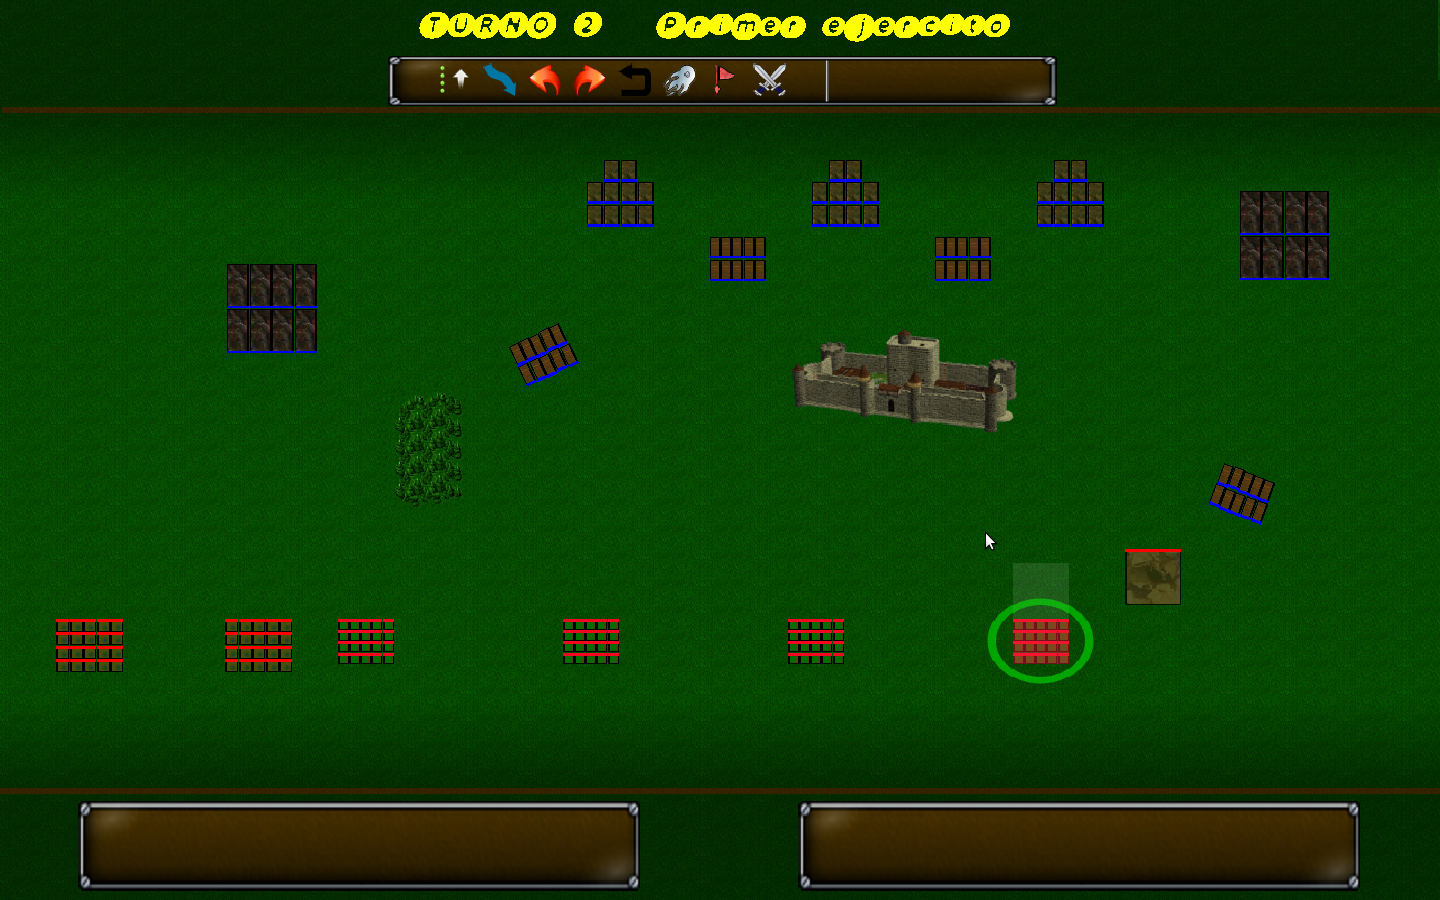
\includegraphics[scale=.2]{imagenes/BatallaGoM.png}
\end{center}
\end{frame}

\section{Juegos de guerra}
\subsection{Taxonomía}
\begin{frame}
  \begin{block}{Aspectos de la guerra}
    \begin{itemize}
    \item Alta estrategía: política
    \item Estrategía: organizativa
    \item Táctica: operacional
    \end{itemize}
  \end{block}

  \begin{block}{Formas de hacer la guerra}
    \begin{itemize}
      \item Paradigma clásico (y fantástico)
      \item Paradigma moderno (y futurista)
    \end{itemize}
  \end{block}

  \begin{block}{Juego de guerra}
    \begin{itemize}
    \item Simulan estos aspectos, en turnos o en tiempo real.
    \item \textit{GoM} es un videojuego 2D libre de táctica militar fantástico
      basado en turnos.
    \end{itemize}
  \end{block}
\end{frame}

\subsection{Afición}
\begin{frame}{Warhammer Fantasy Battles}
  \begin{center}
    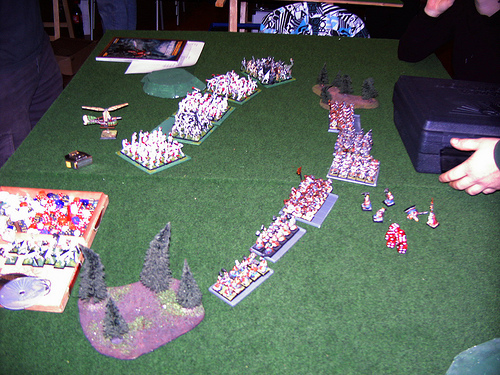
\includegraphics[scale=.4]{imagenes/4058665180_be06e69d7e.jpg}
  \end{center}
\end{frame}

\begin{frame}{Warhammer 40k}
  \begin{center}
    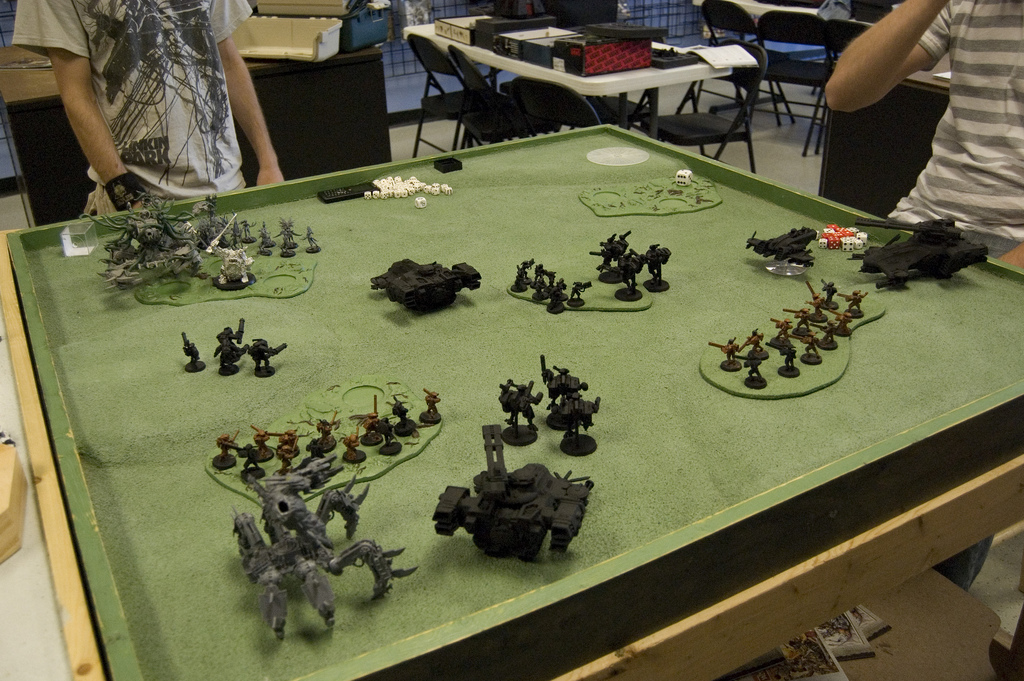
\includegraphics[scale=.7]{imagenes/2593780055_1c7d7ae735_b.jpg}
  \end{center}
\end{frame}

\begin{frame}{Infantilización}
  \begin{center}
    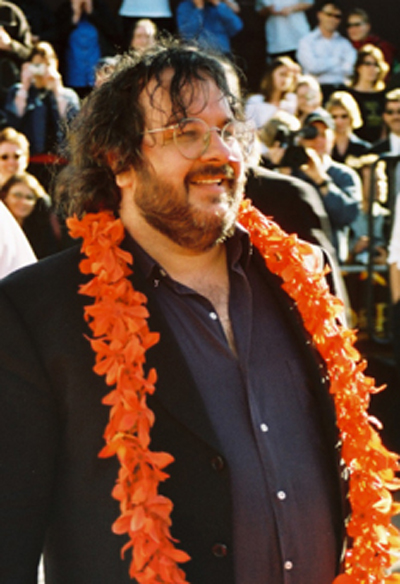
\includegraphics[scale=.3]{imagenes/Peter_Jackson01.jpg}
  \end{center}
\end{frame}

\begin{frame}{Alternativas digitales}
  \begin{minipage}[h]{.35\columnwidth}
    \begin{itemize}
    \item Tiempo real
    \item Alta estrategia
    \end{itemize}
  \end{minipage}
  \begin{minipage}[h]{.6\columnwidth}
    \centering
    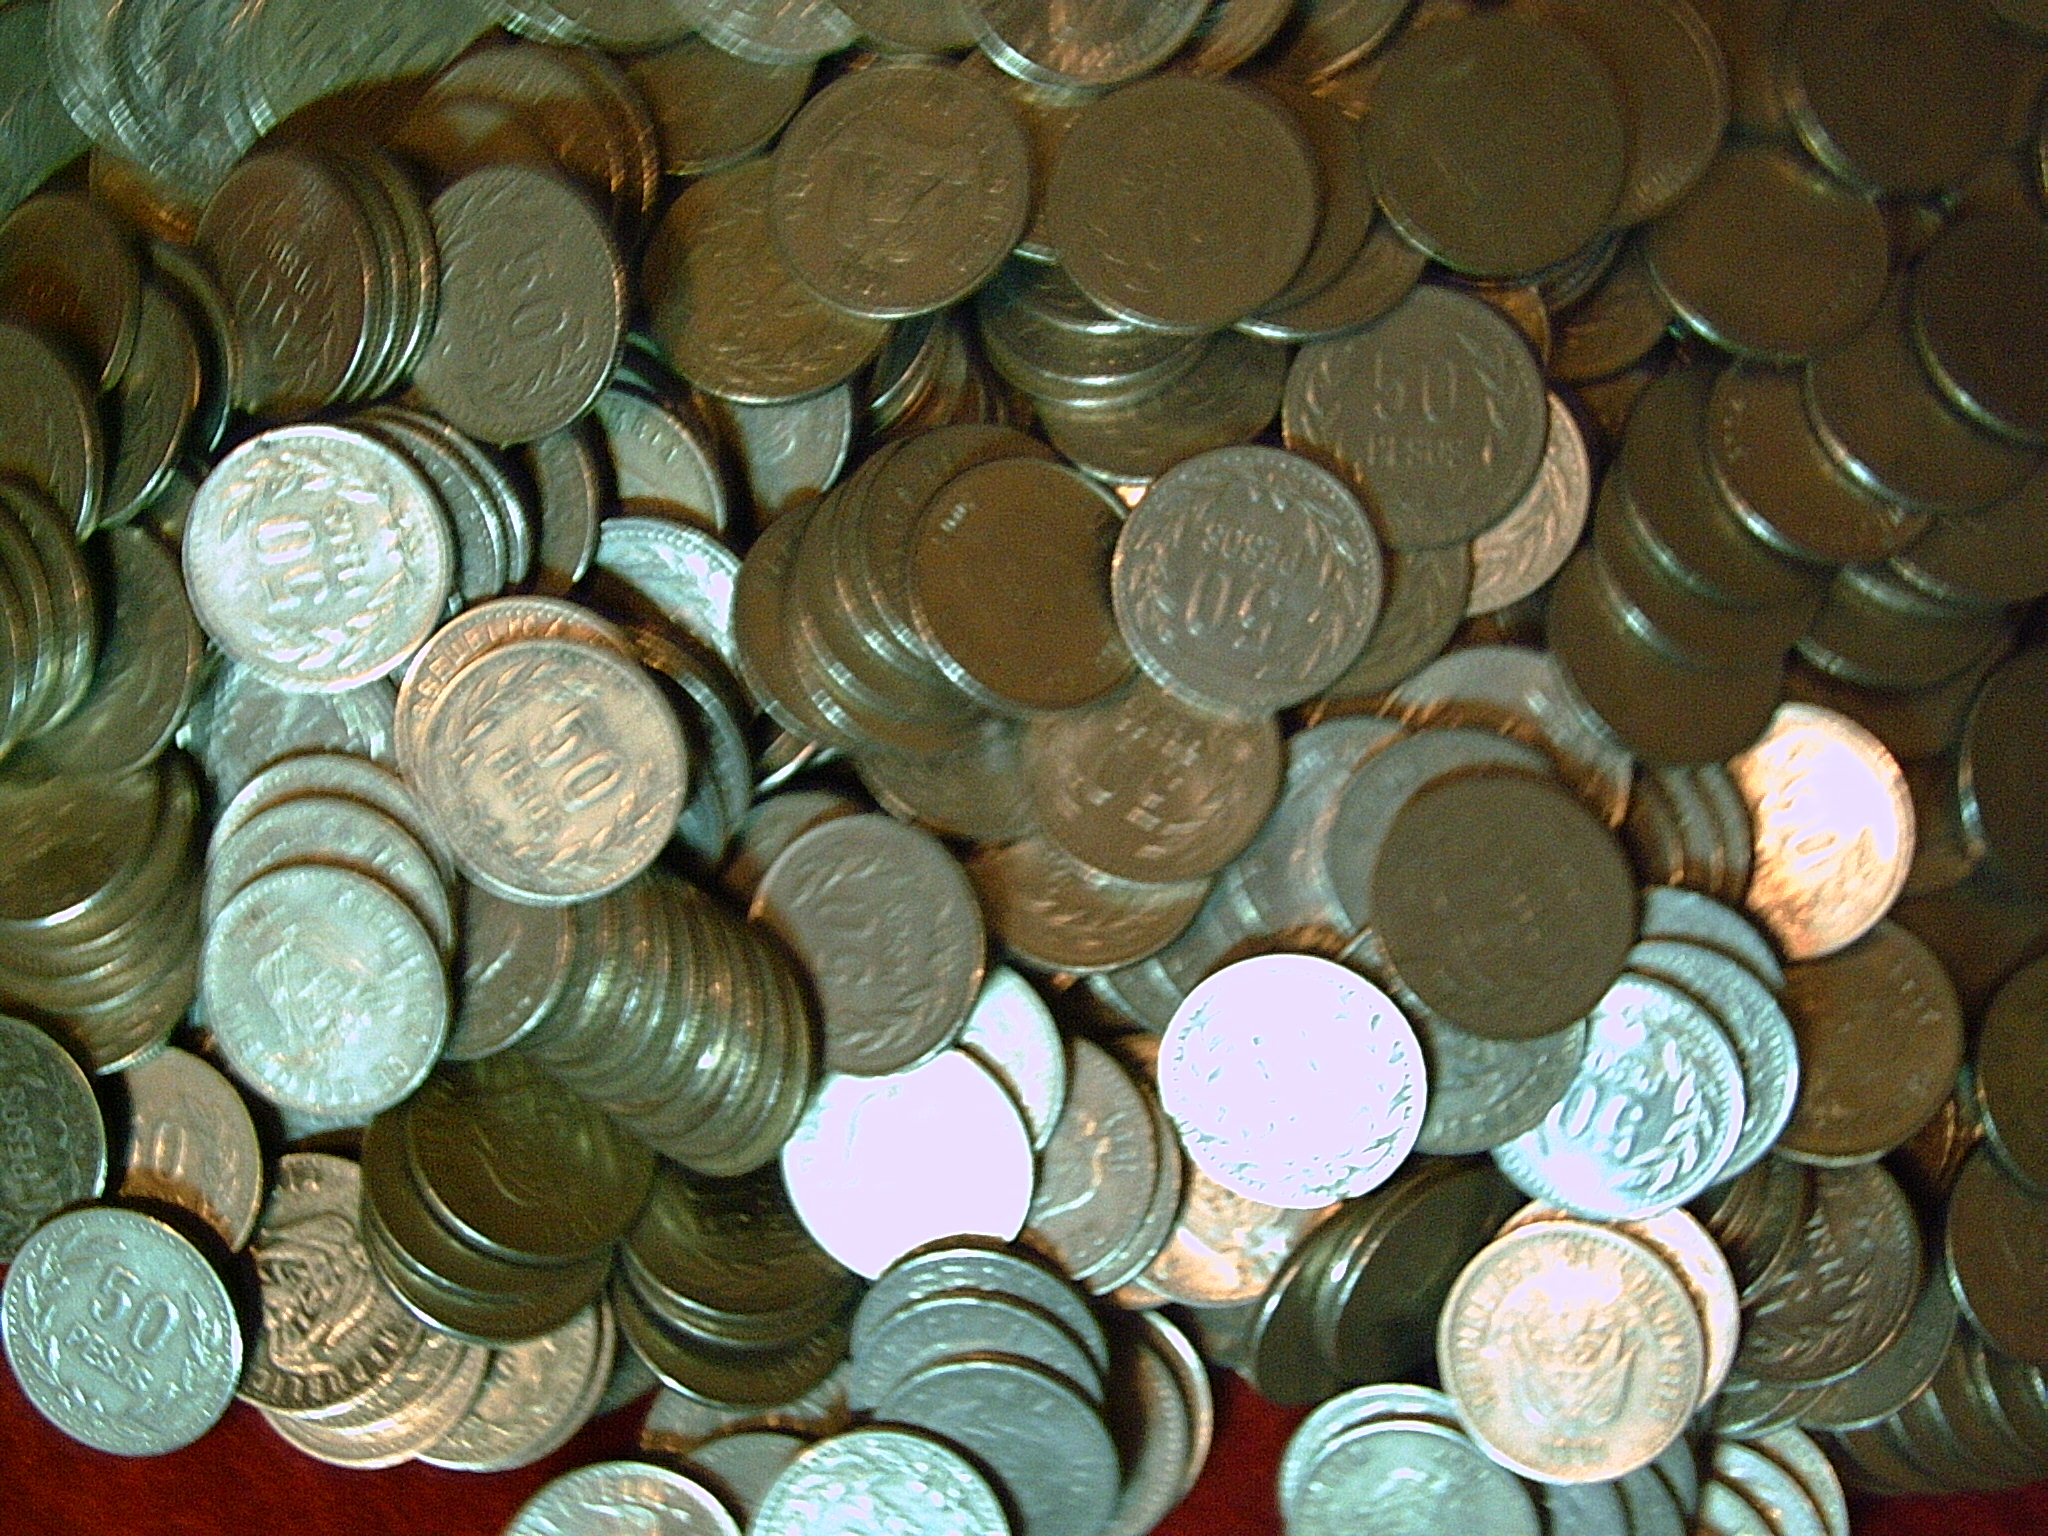
\includegraphics[scale=.07]{imagenes/Dinero_colombia.jpg}
  \end{minipage}
\end{frame}

\section{GoM}
\subsection{Calendario}
\begin{frame}
  \centering
  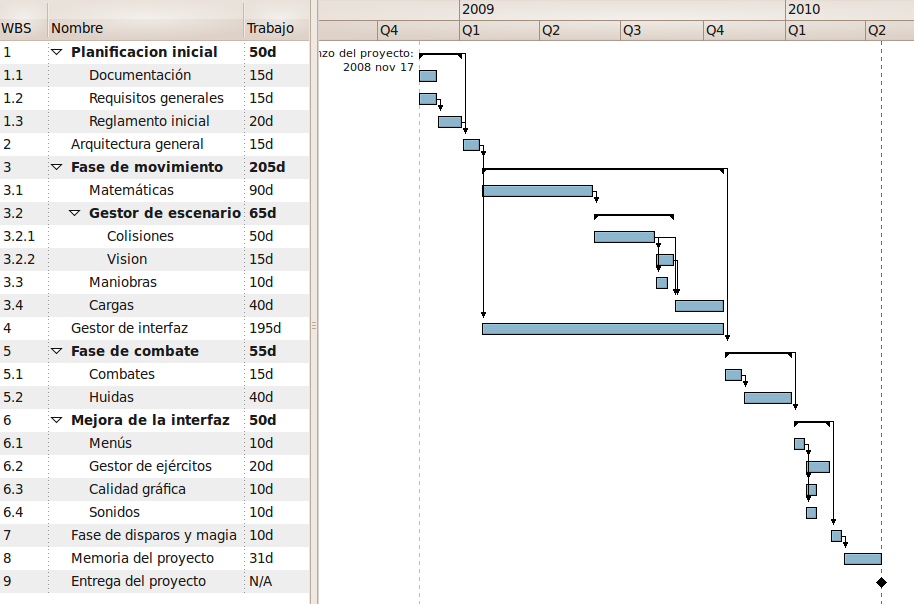
\includegraphics[scale=.35]{imagenes/gGantt.png}
\end{frame}

\subsection{Reglamento}
\begin{frame}
  \begin{block}{Turnos y fases}
    \begin{itemize}
    \item Dos jugadores
    \item Seis turnos de juego
    \item Fase de movimiento: declaración de carga, movimiento de las
      cargas, resto de movimientos
    \item Fase de combate: resolución de combates, efectos de los combates
    \item Fase de disparo
    \end{itemize}
  \end{block}
\end{frame}

\begin{frame}
  \begin{block}{Ejércitos y unidades}
    \begin{itemize}
    \item Dos razas disponibles: humanos y orcos
    \item Ejército: conjunto de unidades de la misma raza
    \item Unidad: conjunto de efectivos iguales
      \begin{itemize}
      \item Formación en bloque
      \item Perfil de atributos
      \end{itemize}
    \end{itemize}
  \end{block}

  \begin{block}{Restricciones}
    \begin{itemize}
    \item Respeto estricto al reglamento
    \item Aleatoriedad
    \item Espacio entre unidades
    \end{itemize}
  \end{block}
\end{frame}

\subsection{Análisis y diseño}
\begin{frame}
  \begin{block}{Observaciones}
    \begin{itemize}
    \item El reglamento es independiente de su visualización
    \item Reglas vs interfaz
    \item Comunicación entre niveles
    \item Acciones de usuario vs cambios de estado
    \item Gestor de ejércitos
    \end{itemize}
  \end{block}
\end{frame}

\begin{frame}{Arquitectura general}
\begin{center}
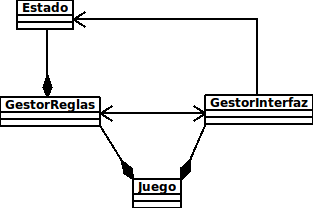
\includegraphics[scale=.9]{imagenes/DiagramaJuego.png}
\end{center}
\end{frame}

\begin{frame}{Gestor de reglas}
\begin{center}
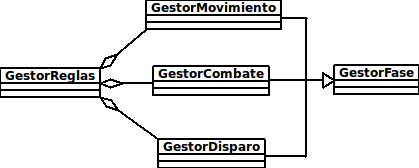
\includegraphics[scale=.9]{imagenes/Reglas.png}
\end{center}
\end{frame}

\begin{frame}{Gestor de interfaz}
\begin{center}
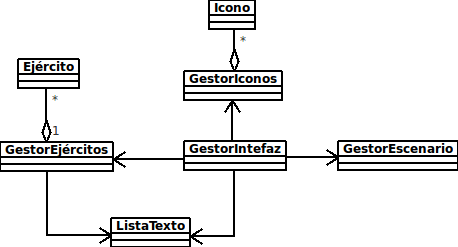
\includegraphics[scale=.8]{imagenes/Interfaz.png}
\end{center}
\end{frame}

\begin{frame}{Gestor de escenario}
\begin{center}
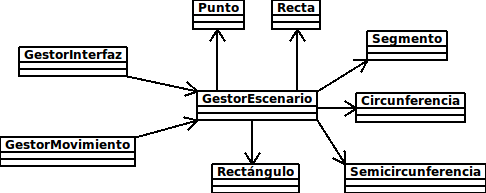
\includegraphics[scale=.8]{imagenes/Escenario.png}
\end{center}
\end{frame}

\subsection{Implementación}
\begin{frame}{Pertenencia de un punto a una figura}
\begin{center}
\begin{tabular}{cc}
\begin{tikzpicture}[scale=2, decoration = {
    markings,
    mark=at position .10 with {\arrow[red, line width = 1.5pt]{>};} ,
    mark=at position .43 with {\arrow[red, line width = 1.5pt]{>}} ,
    mark=at position .76 with {\arrow[red, line width = 1.5pt]{>};} }
  ]
  \draw[gray,postaction={decorate}] (0,0) circle (1cm);
  \draw[thick,blue] (120:1cm) -- (240:1cm) -- (360:1cm) -- cycle;
  \filldraw[green] (120:1cm) circle(1pt);
  \filldraw[green] (240:1cm) circle(1pt);
  \filldraw[green] (360:1cm) circle(1pt);
  \draw (120:1.2cm) node[fill=white] {$A$};
  \draw (240:1.2cm) node[fill=white] {$B$};
  \draw (360:1.2cm) node[fill=white] {$C$};
\end{tikzpicture}
&
\begin{tikzpicture}[scale=2, decoration = {
    markings,
    mark=at position .10 with {\arrow[red, line width = 1.5pt]{<};} ,
    mark=at position .43 with {\arrow[red, line width = 1.5pt]{<}} ,
    mark=at position .76 with {\arrow[red, line width = 1.5pt]{<};} }
  ]
  \draw[gray,postaction={decorate}] (0,0) circle (1cm);
  \draw[thick, blue] (180:1cm) -- (300:1cm) -- (60:1cm) -- cycle;
  \filldraw[green] (180:1cm) circle(1pt);
  \filldraw[green] (300:1cm) circle(1pt);
  \filldraw[green] (60:1cm) circle(1pt);
  \draw (180:1.2cm) node[fill=white] {$A$};
  \draw (300:1.2cm) node[fill=white] {$C$};
  \draw (60:1.2cm) node[fill=white] {$B$};
\end{tikzpicture}
\end{tabular}
\end{center}
\end{frame}

\begin{frame}{Pertenencia de un punto a una figura}
\begin{center}
\[ \vec{u} \times \vec{v} = 
  \begin{vmatrix}u_y & 0 \\v_y & 0 \\\end{vmatrix} \vec{i}
  - \begin{vmatrix}u_x & 0 \\v_x & 0 \\\end{vmatrix} \vec{j}
  + \begin{vmatrix}u_x & u_y \\v_x & v_y \\\end{vmatrix} \vec{k}
 = (u_xv_y - u_yv_x)\vec{k} \]

\begin{tikzpicture}[scale=.9]
\draw[thick,blue] (0,0) -- (2,2) -- (4,0) -- (2,-2) -- cycle;

\filldraw[green] (0,0) circle(1pt);
\filldraw[green] (2,2) circle(1pt);
\filldraw[green] (4,0) circle(1pt);
\filldraw[green] (2,-2) circle(1pt);

\draw (0,-0.6) node {$A$};
\draw (2,2.5) node {$B$};
\draw (4.5,0) node {$C$};
\draw (2,-2.5) node {$D$};

\draw (3,1.7) node[fill=white] {$p$};
\draw[->] (2.8,1.6) -- (1.8,0.6);

\draw [red] (0,0) -- (1.7,0.5);
\draw [red] (2,2) -- (1.7,0.5);
\draw [red] (4,0) -- (1.7,0.5);
\draw [red] (2,-2) -- (1.7,0.5);

\filldraw[green] (1.7,0.5) circle(1pt);

\draw (1.2,0.7) node {$\scriptstyle ABp$};
\draw (2.6,0.7) node {$\scriptstyle BCp$};
\draw (2.5,-0.3) node {$\scriptstyle CDp$};
\draw (1.2,-0.3) node {$\scriptstyle DAp$};
\end{tikzpicture}
\end{center}
\end{frame}

\begin{frame}{Desplazamiento máximo}
\begin{center}
\begin{tikzpicture}[scale=1.5]
\filldraw[rotate=300,blue!30] (0,0) -- (1,0) -- (1,2) -- (0,2) --
cycle;
\filldraw[rotate=300,very thick] (0,0) -- (1,0);
\draw[brown!20!black,->] (.2,.3) node[above] {\tiny{frente}} -- (0.2,-.25);
\filldraw[rotate=345,opacity=.5, green!60] (0.2,1) -- (1.5,1) -- (1.5,2) -- (0.2,2) -- cycle;
\draw[rotate=300,gray,thin] (0,0) -- (1,0) -- (1,-1) -- (0,-1) --
cycle;
\draw[rotate=30,red] (0,0) -- (1.41,0);
\draw[rotate=30,black] (1.41,0)  -- (1.41,-1);
\draw[rotate=30,blue] (0,-0.5) -- (1.41,-0.5);
\draw[rotate=30,blue] (0.7,-0.3) node {$d$};
\filldraw[red,rotate=30] (1.41,0) circle(1pt);
\draw[brown!20!black,->] (-.5, 0) node[above] {\tiny{unidad}} -- (-.5, -.5);
\draw[brown!20!black,->] (1,-1) node[below] {\tiny{desplazamiento}}  --
(1,-.4);
\draw[brown!20!black,->] (0,1.2) node[left] {\tiny{unidad}} -- (.8,1.2);
\end{tikzpicture}
\end{center}
\end{frame}

\begin{frame}{Pivotaje máximo}
\begin{minipage}{.45\columnwidth}
\centering
\begin{tikzpicture}[scale=1.5]
\filldraw[blue!10,rotate=300] (0,0) -- (1,-1) arc (-45:150:1.41cm) --
cycle;
\filldraw[opacity=.7,rotate=300,green!50,draw=black] (0,0) -- (1,0) --
(1,-1) -- (0,-1) -- cycle;
\draw[opacity=.7,red!50!black,rotate=300,thick,->] (0,0) -- (1,-1);
\filldraw[blue!30,rotate=300] (1,0) arc (0:150:1cm) -- (0,0) -- cycle;
\filldraw[very thick,rotate=300] (0,0) -- (1,0);

\filldraw[opacity=.7,rotate=60,green!50,draw=black] (0,0) -- (1,0) -- (1,-1) -- (0,-1) --
cycle;
\draw[red,->,rotate=300] (.5,0) arc (0:119:.5cm);
\filldraw[very thick, rotate=60] (0,0) -- (1,0);
\draw[brown!20!black,->] (-.8,.8) node[above] {\tiny{Área de pivotaje}}
-- (.1,.5);
\draw[brown!20!black,->] (1.2,-1.5) node[below] {\tiny{Área de pivotaje ampliada}}
-- (.8,-1);
\draw[brown!20!black,->] (1.5,1) node[above] {\tiny{Área no controlada}}
  -- (1.2,.3);
\draw[red!70!black,rotate=300] (1,-1) arc (-45:150:1.41cm);
\draw[brown!20!black,->] (-.5,.2) node[above] {\tiny{Frente de la unidad}}
  -- (.08,.2);
\draw[brown!20!black,->] (-.5,.2) -- (.14,-.3);
\end{tikzpicture}
\end{minipage}
\begin{minipage}{.45\columnwidth}
\centering
\begin{tikzpicture}[scale=1.5]
\filldraw[blue!30,rotate=300] (0,0) -- (1,-1) arc (-45:150:1.41cm) --
cycle;
\filldraw[opacity=.5,blue!50, draw=green!40!black,rotate=300] (.4,0) arc(0:56:.4cm) -- (0,0) -- cycle;
\draw[very thick, rotate=300] (0,0) -- (1,0);
\filldraw[opacity=.5,rotate=300,green!50,draw=black] (0,0) -- (1,0) --
(1,-1) -- (0,-1) -- cycle;
\filldraw[opacity=.5,green!50,draw=black] (1,.5) -- (2,1.5) --
(3,0.5) -- (2,-.5) -- cycle;
\filldraw[red] (1.41,.1) circle(1.5pt);
\draw[red!30!black] (1.41,.1) circle(.2cm);
\draw[blue] (0,0) -- (1.4,-.1);

\draw[brown!20!black,->] (1.8,-1) node[below] {\tiny{Área de espacio
    entre unidades}}-- (1.45,-.03);
\draw[brown!20!black,->] (-.6,.7) node[above] {\tiny{Ángulo de pivotaje}}-- (.2,-.15);
\end{tikzpicture}
\end{minipage}
\end{frame}

\begin{frame}{Visión}
\begin{center}
\begin{tikzpicture}[
  scale=1.5,
  rotate=300,
  unidad/.style={opacity=.5,green!50,draw=black},
  area/.style={opacity=.5,blue!50, draw=green!40!black},
  descripcion/.style={brown!20!black,->},
  ]
\coordinate (A) at (0,1);
\coordinate (B) at (1.5,1);
\coordinate (C) at (1.5,0);
\coordinate (D) at (0,0);

\coordinate (a) at (.5,2.5);
\coordinate (b) at (1.2,2.5);
\coordinate (c) at (1.2,3.2);
\coordinate (d) at (.5,3.2);

\coordinate (REF) at (a);
\coordinate (CENTRO) at (.75,1);

\filldraw[area] (0.4,1) -- (0.2,1) -- ({.5 + .2*cos(30)}, {2.5 + .2*sin(30)})--
+({.2*cos(30)}, {.2*sin(30)}) -- cycle;

\filldraw[unidad] (A) rectangle (C);

%No se por que no funciona girar coordenadas (c).
\filldraw[unidad,rotate around={30:(REF)}] (a) rectangle (1.2,3.2);

\coordinate (alfa) at (.9,1.5);
\coordinate (beta) at (1.4,2.4);

\filldraw[unidad,rotate around={10:(alfa)}] (alfa) rectangle (beta);

\filldraw[unidad,rotate around={30:(-.5,2.4)}] (0,1.5) rectangle
(-.5,2.4);

\draw[descripcion] (-.5,.5) node[above]{\tiny{Unidad actual}} --
(.5,.5);
\draw[descripcion] (-.5,1.5) node[above]{\tiny{Haz de visión}} --
(.45,1.5);

\coordinate (refunidades) at (1.8,1);

\draw[descripcion] (refunidades) node[below]{\tiny{Otras unidades}} --
(1.11,1.7);

\draw[descripcion] (refunidades) -- (0,1.8);

\draw[very thick] (A) -- (B);

\coordinate (refunidadobjetivo) at (0,3.35);

\draw[descripcion] (refunidadobjetivo) node[above]{\tiny{Unidad
    objetivo}} -- (.6,3);
\end{tikzpicture}
\end{center}
\end{frame}

\begin{frame}{Visión}
\begin{center}
\begin{tikzpicture}[
  scale=1.5,
  rotate=300,
  unidad/.style={opacity=.5,green!50,draw=black},
  area/.style={opacity=.5,blue!50, draw=green!40!black},
  descripcion/.style={brown!20!black,->}
  ]
\coordinate (A) at (0,1);
\coordinate (B) at (1.5,1);
\coordinate (C) at (1.5,0);
\coordinate (D) at (0,0);

\coordinate (a) at (.5,2.5);
\coordinate (b) at (1.2,2.5);
\coordinate (c) at (1.2,3.2);
\coordinate (d) at (.5,3.2);

\coordinate (REF) at (a);
\coordinate (CENTRO) at (.75,1);

\filldraw[unidad] (A) rectangle (C);

%No se por que no funcioan girar coordenadas (c) no funciona.
\filldraw[unidad,rotate around={30:(REF)}] (a) rectangle (1.2,3.2);
\draw[very thick] (A)--(B);

\filldraw[red,rotate around={30:(REF)}] (CENTRO) circle(1pt) -- (intersection of a--1.2,3.2
and 1.2,2.5--.5,3.2) circle(1pt);
\draw[opacity=.5,green, rotate around={30:(REF)}] (a)--(1.2,3.2);
\draw[opacity=.5,green, rotate around={30:(REF)}] (1.2,2.5)--(.5,3.2);

\draw[blue, rotate around={30:(REF)}] (a)--(1.2,2.5);
\draw[area] (CENTRO)--(a);
\draw[area, rotate around={30:(REF)}] (CENTRO) -- (1.2,2.5);

\draw[descripcion] (-.5,.5) node[above]{\tiny{Unidad actual}} --
(.5,.5);

\coordinate (refunidadobjetivo) at (0,3.35);

\draw[descripcion] (refunidadobjetivo) node[above]{\tiny{Unidad
    objetivo}} -- (.6,3);

\draw[descripcion] (1.5,2) node[below]{\tiny{Recta discriminatoria}}
-- (.74, 1.7);
\end{tikzpicture}
\end{center}
\end{frame}

\begin{frame}{Visión}
\begin{center}
\begin{tikzpicture}[
  scale=1.5,
  rotate=300,
  unidad/.style={opacity=.5,green!50,draw=black},
  area/.style={opacity=.5,blue!50, draw=green!40!black},
  descripcion/.style={brown!20!black,->},
  decoration = {
    markings,
    mark=at position .50 with {\arrow[red, line width = 1.5pt]{>};} }
  ]
\coordinate (A) at (0,1);
\coordinate (B) at (1.5,1);
\coordinate (C) at (1.5,0);
\coordinate (D) at (0,0);

\coordinate (a) at (.5,2.5);
\coordinate (b) at (1.2,2.5);
\coordinate (c) at (1.2,3.2);
\coordinate (d) at (.5,3.2);

\coordinate (REF) at (a);
\coordinate (CENTRO) at (.75,1);

\filldraw[area,opacity=.3,rotate around={30:(REF)}] (CENTRO) -- (.5,3.2) --
(1.2,2.5) -- cycle;
\filldraw[area,black!80,rotate around={30:(REF)}] (.5,3.2) --
(1.2,2.5) -- (1.2,3.2) -- cycle;

\filldraw[unidad] (A) rectangle (C);

%No se por que no funcioan girar coordenadas (c) no funciona.
\filldraw[unidad,rotate around={30:(REF)}] (a) rectangle (1.2,3.2);
\draw[very thick] (A)--(B);

\draw[red, rotate around={30:(REF)}] (1.2,2.5)--(.5,3.2);

\draw[blue, rotate around={30:(REF)}] (a)--(1.2,2.5);
\draw[blue, rotate around={30:(REF)}] (a)--(.5,3.2);
\draw[red, rotate around={30:(REF)},postaction={decorate}] (CENTRO) --
(1.2,2.5);

\draw[descripcion] (1.5,2) node[below]{\tiny{Área de referencia}}
-- (.74, 2);
\draw[descripcion] (0,3.5) node[above]{\tiny{Área oculta}} --
(.6,3.15);
\draw[descripcion] (-.27,1.4) node[above]{\tiny{Diagonal
    discriminatoria}} -- (.63,2.96);
\end{tikzpicture}
\end{center}
\end{frame}

\begin{frame}{Movimiento de huida}
\begin{center}
\begin{tikzpicture}[
  scale=1.2,
  rotate=250,
  unidad/.style={opacity=.5,green!50,draw=black},
  area/.style={opacity=.5,blue!50, draw=green!40!black},
  fondo/.style={blue!10},
  descripcion/.style={brown!20!black,->}
  ]

\filldraw[fondo] (0,1) rectangle (1,7);
\filldraw[area] (0,1) rectangle (1,3.5);
\filldraw[unidad] (0,0) rectangle (1,1);
\draw[very thick] (0,1) -- (1,1);
\filldraw[unidad, rotate around={30:(-.2,2.5)}] (-.2,2.5) rectangle
(.7,3);
\filldraw[unidad, rotate around={160:(1.4,4.2)}] (1.4,4.2) rectangle
(2.3,4.7);
\filldraw[unidad, rotate around={150:(.5,6)}] (.5,6) rectangle
(1.2,5.4);

\draw[red] (0,2.6) -- (1,2.6);
\draw[red] (0,3.4) -- (1,3.4);
\draw[red] (0,3.8) -- (1,3.8);
\draw[red] (0,4.53) -- (1,4.53);
\draw[red] (0,5.95) -- (1,5.98);
\draw[red] (0,6.9) -- (1,6.9);

\draw[descripcion] (-.5,.5) node[above]{\tiny{Unidad de huida}} --
(.5,.5);
\draw[descripcion] (-.5,4.43) node[above]{\tiny{Espacio libre}}
-- (.3,3.6);
\draw[descripcion] (-.5,4.43) -- (.5,5.25);
\draw[descripcion] (1.7,5) node[below]{\tiny{Unidades a esquivar}} --
(.3, 6.5);
\draw[descripcion] (1.7,5) -- (.8,4.2);
\draw[descripcion] (1.7,5) -- (.3,3);
\draw[descripcion] (-.8,3.5) node[above]{\tiny{Límite de huida}}--
(-.1,3.5);
\end{tikzpicture}
\end{center}
\end{frame}

\section{Conclusiones}
\begin{frame}
\begin{block}{Objetivos conseguidos}
\begin{itemize}
\item Videojuego libre de táctica militar por turnos de corte fantástico
\item Reglamento suficiente y complejo
\item Mejores conocimientos sobre programación multimedia
\end{itemize}
\end{block}

\begin{block}{Experiencia ganada}
\begin{itemize}
\item Abstracción
\item Ingeniería del software
\item Organización modular
\end{itemize}
\end{block}
\end{frame}

\begin{frame}
\begin{block}{Mejoras futuras}
\begin{itemize}
\item Inteligencia artificial
\item 3D
\item Historia de la guerra
\item Manejador de reglamentos
\item Herramienta de modelado de miniaturas
\end{itemize}
\end{block}
\end{frame}

\begin{frame}
  \begin{center}
    \Huge{Gracias}
    \vfill
    \LARGE {Demostración}
    \vfill
    \LARGE {Preguntas}
    \vfill
    \large{\url{https://forja.rediris.es/projects/gom/}}
  \end{center}
\end{frame}


\end{document}